%%%%%%%%%%%%%%%%%%%%%%%%%%%%%%%%%%%%%%%%%
% University Assignment Title Page 
% LaTeX Template
\title{Template báo cáo KHTN}
%----------------------------------------------------------------------------------------
%	PACKAGES AND OTHER DOCUMENT CONFIGURATIONS
%----------------------------------------------------------------------------------------

\documentclass[12pt]{article}
\usepackage[T5]{fontenc}
\usepackage[utf8]{inputenc}
\usepackage[vietnamese,english]{babel}
\usepackage{amsmath}
\usepackage{graphicx}
\usepackage[colorinlistoftodos]{todonotes}
\usepackage{listings}
\usepackage{hyperref}
\usepackage{multirow}
\usepackage{tabularx}
\hypersetup{
    colorlinks=true,
    linkcolor=black,
    filecolor=magenta,      
    urlcolor=cyan,
}
\usepackage{listings}
\usepackage{xcolor}

% Thiết lập màu sắc cho code
\definecolor{codegreen}{rgb}{0.2,0.8,0.2}
\definecolor{codegray}{rgb}{0.5,0.5,0.5}
\definecolor{codepurple}{rgb}{0.58,0,0.82}
\definecolor{backcolour}{rgb}{0.95,0.95,0.92}

% Thiết lập cấu hình cho gói lệnh listings
\lstdefinestyle{mystyle}{
    backgroundcolor=\color{backcolour},
    commentstyle=\color{codegreen},
    keywordstyle=\color{magenta},
    numberstyle=\tiny\color{codegray},
    stringstyle=\color{codepurple},
    basicstyle=\ttfamily\footnotesize,
    breakatwhitespace=false,
    breaklines=true,
    captionpos=b,
    keepspaces=true,
    numbers=left,
    numbersep=5pt,
    showspaces=false,
    showstringspaces=false,
    showtabs=false,
    tabsize=2
}

% Sử dụng gói lệnh listings và cấu hình cho code Python
\lstset{style=mystyle, language=Python}
\usepackage[a4paper, left=2cm, right=2cm, top = 2cm, bottom = 2cm]{geometry}
\begin{titlepage}

\begin{document}

\newcommand{\HRule}{\rule{\linewidth}{1mm}} % Defines a new command for the horizontal lines, change thickness here

\begin{center}

%----------------------------------------------------------------------------------------
%   LOGO SECTION
%----------------------------------------------------------------------------------------


\includegraphics[width=3cm]{logo/rsz_3logo-khtn.png}\\[1cm] % Include a department/university logo - this will require the graphicx package

%----------------------------------------------------------------------------------------
%   HEADING SECTIONS
%----------------------------------------------------------------------------------------

\textsc{\LARGE UNIVERSITY OF SCIENCE - VNUHCM}\\[1cm]
\textsc{\large Applied Linear Algebra and Mathematical Statistics }\\[0.5cm]
\textsc{\Large 21\_5}\\[1.5cm]


%----------------------------------------------------------------------------------------
%   TITLE SECTION
%----------------------------------------------------------------------------------------

\HRule \\[0.5cm]
{ \huge \bfseries Maximum Likelihood Estimation }\\[0.2cm]
\HRule \\[1.5cm]

\tableofcontents

%----------------------------------------------------------------------------------------
%   AUTHOR SECTION
%----------------------------------------------------------------------------------------
\begin{center}
\makebox[\textwidth]{%
\begin{tabular}{@{} c @{}}
\begin{minipage}{0.45\textwidth}
\begin{flushleft} \large
\emph{Students}\\[0.2cm]
Thai Tan Tran -- 21120553 \\
Huu Thuan Nguyen -- 21120566
\end{flushleft}
\end{minipage}
\end{tabular}
\hfill
\begin{tabular}{@{} c @{}}
\begin{minipage}{0.45\textwidth}
\begin{flushright} \large
\emph{Teacher} \\[0.2cm]
PhD. Ha Son Tran
\end{flushright}
\end{minipage}
\end{tabular}%
}
\end{center}
\end{center}

\vfill % Fill the rest of the page with whitespace

\section{Lý thuyết}

\subsection{Giới thiệu}

{\fontsize{13}{16}\selectfont
\setlength{\parskip}{0.3cm}
Các mô hình thống kê thường kết hợp nhiều phân phối xác suất để mô phỏng và phân tích dữ liệu. Việc tìm các tham số của phân phối xác suất (ký hiệu là $\theta$) giúp xây dựng mô hình thống kê chính xác và phù hợp với dữ liệu quan sát. Thông qua quá trình ước lượng tham số, chúng ta có thể sử dụng mô hình để dự đoán, suy luận và khám phá thêm thông tin về dữ liệu và quá trình sinh dữ liệu. Ví dụ, trong phân phối Bernoulli, tham số cần tìm là $p$, trong phân phối chuẩn (Gaussian), tham số cần tìm là trung bình $\mu$ và phương sai $\sigma^2$,...

\noindent Phương pháp ước lượng hợp lý cực đại (maximum likelihood estimation) là phương pháp cơ bản và phổ biến nhất trong việc ước lượng các tham số của một mô hình dựa trên dữ liệu quan sát được.
}

\subsection{Ý tưởng}
{\fontsize{13}{16}\selectfont
\setlength{\parskip}{0.3cm}
Giả sử có các điểm dữ liệu $X_1, X_2,...,X_n$ và chúng tuân theo một phân phối xác suất nào đó được mô tả bởi bộ tham số (ký hiệu là $\theta$). 

\noindent Phương pháp ước lượng hợp lý cực đại (maximum likelihood estimation - MLE) giúp ta ước lượng được bộ tham số $\theta$ sao cho: 
$$\theta = \max_{\theta} P(X_1, X_2,...,X_n | \theta)$$

\noindent Như đã biết, $P(X_1 | \theta)$ là xác suất xảy ra dữ liệu $X_1$, vì thế $P(X_1, X_2,...,X_n | \theta)$ là xác suất xảy ra đồng thời các dữ liệu $X_1, X_2,...,X_n$, xác suất này còn gọi là likelihood. Bởi vì các dữ liệu được xảy ra rồi, do đó ta cần phải tìm cách để xác suất này xảy ra càng cao càng tốt, đó cũng chính là lý do tại sao cần phải đi tìm bộ tham số để likelihood lớn nhất.

\noindent Tuy nhiên, việc giải trực tiếp biểu thức trên là rất khó khăn nên ta giả sử các điểm dữ liệu $X_n$ độc lập với nhau. Khi đó:

$$P(X_1, X_2,...,X_n | \theta) = \prod_{k = 1}^{n}P(X_k|\theta)$$

\noindent Vậy bài toán ban đầu có thể đưa về bài toán tối ưu sau:

$$\theta = \max_{\theta}\prod_{k = 1}^{n}P(X_k|\theta)$$

\noindent Tối ưu hóa một tích thường khó hơn một tổng, vì vậy để đơn giản hóa bài toán trên ta lấy $\log$ hai vế (vì hàm $\log$ là hàm đồng biến trên tập xác định của nó nên $\log$ của hàm số lớn nhất thì hàm số cũng lớn nhất).

\noindent Bài toán Maximum Likelihood được đưa về bài toán Maximum Log-Likelihood:

$$\theta = \max_{\theta}\sum_{k = 1}^{n}\log(P(X_k|\theta))$$

\noindent Để giải bài toán trên, có thể đạo hàm tìm được cực trị theo từng biến. Với từng phân phối xác suất sẽ có kết quả khác nhau, sẽ được đề cập kĩ trong phần Ứng dụng.

\section{Ứng dụng}
\subsection{Phân phối chuẩn}
\subsubsection{Bài toán}
{\fontsize{13}{16}\selectfont
\setlength{\parskip}{0.3cm}
Giả sử các điểm dữ liệu $X_1, X_2,...,X_n$ tuân theo phân phối chuẩn (Gaussian), tức tham số cần ước lượng là trung bình $\mu$ và phương sai $\sigma^2$. Và ta cũng có:
$$P(X_k|\mu, \sigma^2) = \frac{1}{\sqrt{2\pi\sigma^2}}\exp{\frac{-1}{2\sigma^2}(X_k-\mu)^2}$$

\noindent Để thuận tiện thì thay vì lấy $\log$ (theo cơ số 10) thì ta sẽ lấy $\log$ theo cơ số $e$, tức lấy $\ln$.

\noindent Khi đó
$$\ln(P(X_k|\theta) = -\ln{(\sqrt{2\pi})}-ln{(\sigma)} - \frac{1}{2\sigma^2}(X_k-\mu)^2$$

\noindent Bỏ đi lượng $-\ln{(\sqrt{2\pi})}$ vì nó không ảnh hưởng đến bài toán, khi đó ta có
$$A=\sum_{k = 1}^{n}\ln(P(X_k|\mu, \sigma^2)) = -nln{(\sigma)} - \frac{\sum_{k = 1}^{n}(X_k-\mu)^2}{2\sigma^2}$$

\noindent Vậy để tìm $\mu$ và $\sigma^2$ chỉ cần giải hệ phương trình đạo hàm
\setlength{\jot}{10pt}
\[
\begin{cases}
     \frac{\partial A}{\partial\mu} = 0\\
     \frac{\partial A}{\partial\sigma} = 0
\end{cases}
\quad \Leftrightarrow \quad
\begin{cases}
\frac{1}{\sigma^2}\sum_{k = 1}^{n}(X_k-\mu) = 0 \\
-\frac{n}{\sigma} + \frac{1}{\sigma^3}\sum_{k = 1}^{n}(X_k-\mu)^2 = 0 \\
\end{cases}
\quad \Leftrightarrow \quad
\begin{cases}
\mu =  \frac{\sum_{k = 1}^{n}X_k}{n}\\
\sigma^2 =  \frac{\sum_{k = 1}^{n}(X_k-\mu)^2}{n}\\
\end{cases}
\]
\subsubsection{Ứng dụng vào mô hình Linear Regression}
\noindent Ta có thể áp dụng phân phối chuẩn trong mô hình Linear Regression. Giả sử mô hình có dạng $y_k = \alpha + \beta x_k + \epsilon_k$, trong đó sai số $\epsilon$ tuân theo phân phối chuẩn với trung bình ($\mu$) bằng 0 (để sai số tối ưu nhất thì trung bình bằng 0). Ta sẽ ước lượng để tìm các tham số còn lại sao cho tối ưu nhất (Sẽ khác với bài toán trên một chút vì đã biết trước $\mu = 0$).

\noindent Tương tự như bài toán trên, ta cần tối ưu hàm sau
$$A=\sum_{k = 1}^{n}\ln(P(\epsilon_k|\sigma^2)) = -nln{(\sigma)} - \frac{\sum_{k = 1}^{n}\epsilon_k^2}{2\sigma^2}$$

\noindent Mặt khác ta có $\epsilon_k = y_k - (\alpha + \beta x_k)$

\noindent Vậy $$A = -nln{(\sigma)} - \frac{\sum_{k = 1}^{n}(y_k - (\alpha + \beta x_k))^2}{2\sigma^2}$$

\noindent Đạo hàm hàm số trên để tìm các tham số tương ứng, được
$$\beta =\frac{\sum_{k = 1}^{n}x_k \sum_{k = 1}^{n}y_k-n\sum_{k = 1}^{n}x_k y_k}{\sum_{k = 1}^{n}x_k \sum_{k = 1}^{n}x_k-n\sum_{k = 1}^{n}x_k^2}$$
$$\alpha = \frac{\sum_{k = 1}^{n}y_k - \beta \sum_{k = 1}^{n}x_k}{n}$$
$$\sigma^2 = \frac{1}{n}\sum_{k = 1}^{n}(y_k-(\alpha + \beta x_k))^2$$

\noindent Tuy nhiên, mô hình trên chỉ có một biến độc lập, nếu bài toán Linear Regression có nhiều biến thì việc đạo hàm cho từng biến sẽ rất khó khăn, thay vào đó thư viện scipy.optimize trong Python cung cấp sẵn một hàm (minimize) để tìm giá trị nhỏ nhất của hàm số, lúc này chỉ cần viết hàm trả về biểu thức $-A$ rồi truyền nó vào hàm minimize.

\subsubsection{Thử nghiệm trên dataset thực tế}
\noindent Xét một dataset (Advertsing.csv) được mô tả như sau: 

- Có các cột "ID", "TV", "Radio", "Newspaper", "Sales". 

- Trong đó cột "ID" chỉ số thứ tự của data.

- "TV", "Radio", "Newspaper" lần lượt cho biết chi phí quảng cáo trên các phương tiện truyền thông là TV, Radio, Newspaper.

- "Sales" cho biết doanh số bán hàng.

\noindent Import thư viện và đọc data từ file
\begin{lstlisting}
import numpy as np
import pandas as pd
from scipy.optimize import minimize

# Read file Advertising.csv
data = pd.read_csv("Advertising.csv")

# Prepare data
x = data[["TV", "Radio", "Newspaper"]].values
y = data["Sales"].values
\end{lstlisting}

\noindent Hàm số cần minimize (lưu ý rằng để buộc điều kiện $\sigma >=0$ thì ta cho hàm số theo biến $sigma\_sqr$)
\begin{lstlisting}
def log_likelihood(params, x, y):
    sigma = params[0]
    alpha = params[1]
    beta = params[2:]
    n = len(x)
    sigma_sqr = sigma**2
    return 0.5 * n * np.log(sigma_sqr) + np.sum((y - (alpha + np.dot(x, beta)))**2) / (2 * sigma_sqr)
\end{lstlisting}

\noindent Tối ưu hóa bằng hàm minimize của thư viện scipy.optimize
\begin{lstlisting}
result = minimize(log_likelihood, np.ones(X.shape[1] + 2), args=(x, y))
\end{lstlisting}

\noindent In kết quả
\begin{lstlisting}
print("sigma^2 = ", result.x[0]**2)
print("alpha = ", result.x[1])
print("beta = ", result.x[2:])
\end{lstlisting}
\noindent Kết quả
\begin{verbatim}
    sigma^2 =  2.78412629348835
    alpha =  2.938894141227282
    beta =  [ 0.04576462  0.18853001 -0.00103751]
\end{verbatim}
\subsection{Phân phối Bernoulli}
\subsubsection{Bài toán}
\fontsize{13}{16}\selectfont
\setlength{\parskip}{0.3cm}
Giả sử các điểm dữ liệu $X_1, X_2,...,X_n$ tuân theo phân phối Bernoulli, tức tham số cần ước lượng $p (0 \leq p \leq 1)$. Và ta cũng có:
$$P(X_k|p) = p^{X_k}(1-p)^{1-X_k}$$
Vậy ta cần tìm
$$p = \max_{0\leq p \leq1}\sum_{k = 1}^{n}\log(P(X_k|p)) = \max_{0\leq p \leq 1}\sum_{k = 1}^{n}\log(p^{X_k}(1-p)^{1-X_k})=\max_{0\leq p \leq 1}(\log(p)\sum_{k = 1}^{n}X_k + \log(1-p)(n-\sum_{k = 1}^{n}X_k)) $$
Giải bài toán trên bằng cách cho đạo hàm bằng 0. Khi đó $p$ là nghiệm của phương trình
$$\frac{\sum_{k = 1}^{n}X_k}{p} = \frac{n-\sum_{k = 1}^{n}X_k}{1-p} \Leftrightarrow p = \frac{\sum_{k = 1}^{n}X_k}{n}$$
\subsubsection{Ứng dụng vào mô hình Logistic Regression}
\fontsize{13}{16}\selectfont
\setlength{\parskip}{0.3cm}
Mô hình phân loại dựa vào hàm sigmoid có dạng
$$\sigma(x) = \frac{1}{1+e^{-x}}$$
Với mô hình Linear Regression, với bộ dữ liệu training đầu vào $w = (1, x_1, x_2)$ ta thu được hàm hồi quy 
$$\hat{y} = w_0 + w_1x_1 + w_2x_2 = w^T x$$
Chuyển tiếp giá trị này qua hàm Sigmoid để dự báo xác suất và tạo tính phi tuyển cho mô hình hồi qui
$$P(y=1|x;w)=\sigma(w^T x) = \frac{1}{1+e^{-w^T x}}$$
Lựa chọn ngưỡng xác suất là 0.5 làm threshold, dự báo nhãn là
\begin{equation}
\begin{cases}
0 \text{ nếu } P(y=1|x;w) \leq 0.5 \\
1 \text{ nếu } P(y=1|x;w) > 0.5
\end{cases}
\end{equation}
Bài toán phân loại tuân theo phân phối Bernoulli. Xác suất xảy ra điểm $x_i$ theo hàm sigmoid

\begin{equation}
\begin{cases}
P(y=1|x) = \sigma(w^T x_i)\\
P(y=0|x;w) = 1 - \sigma(w^T x_i)
\end{cases}
\end{equation}
Như vậy ta có thể tổng quát hóa cho một mẫu có cả hai trường hợp $\{0,1\}$ là
$$P(y_i|x_i;w)=P(y=1)^{y_i}(1-P(y=1))^{1-y_1}$$
Giả sử các quan sát trong bộ dữ liệu độc lập. Khi đó giống như trong phần ý tưởng, ta cần xác suất sau càng cao càng tốt
$$P(y|X;w) = \prod_{i=1}^{n}P(y_i|x_i;w)$$
Cũng như phép biến đổi ở bài trên, ta cần đánh giá
$$\max_{w} \sum_{i=1}^{n}(y_i\log(P(y_i=1))+(1-y_i)\log(1-P(y_i=1)))$$
Đặt $\hat{y}_i = P(y_i=1)$ là ước lượng xác suất tại điểm $x_i$. Thực hiện phép biển đổi ta đưa về bài toán sau
$$\min_{w} \sum_{i=1}^{n}-(y_i\log(\hat{y}_i)+(1-y_i)\log(1-\hat{y}_i))$$
Đây cũng chính là hàm mất mát, hay còn gọi là Cross Entropy. Giá trị hàm mất mát này càng nhỏ nếu hai phân phối xác suất càng gần nhau, hay $y = \hat{y}$.

\noindent Để giải bài toán này, ta có thể sử dụng phương pháp Gradient Descent. Vì bài báo cáo chỉ trong khuôn khổ của phương pháp Maximum Likelihood Estimation nên ta không bàn về cách giải từ bước này trở về sau.
\subsubsection{Thử nghiệm trên dataset thực tế}
Xét một dataset (data\_classification.csv) được mô tả như sau:

- Có ba cột "HoursStudy", "HoursSleep", "Result".

- Cột HoursStudy là số giờ một học sinh dùng để học trong một ngày.

- Cột HoursSleep là số giờ một học sinh dùng để ngủ trong một ngày.

- Cột Result cho biết kết quả học sinh đó có đậu kì thi hay không (1-Đậu, 0-Rớt).

\noindent Import thư viện và đọc data từ file
\begin{lstlisting}
import pandas as pd
import numpy as np
import matplotlib.pyplot as plt

data = pd.read_csv("data_classification.csv")
X = data[["HoursStudy", "HoursSleep"]].values
y = data["Result"].values
\end{lstlisting}

\noindent Biểu diễn các điểm dữ liệu
\begin{lstlisting}
for item in data.values:
    if item[2] == 0:
        dat_SoGioHoc.append(item[0])
        dat_SoGioNgu.append(item[1])
    else:
        rot_SoGioHoc.append(item[0])
        rot_SoGioNgu.append(item[1])
    
plt.scatter(dat_SoGioHoc, dat_SoGioNgu, marker = 'o', c='b')
plt.scatter(rot_SoGioHoc, rot_SoGioNgu, marker = 's', c='r')
plt.show()
\end{lstlisting}
\noindent Chạy hàm $plt.show()$
\begin{figure}[htbp]
  \centering
  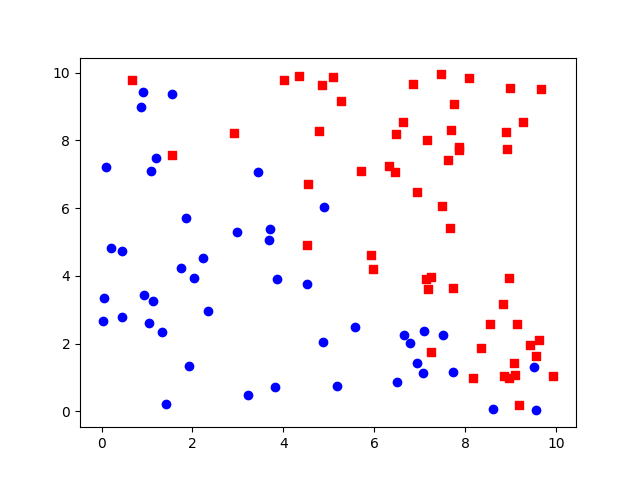
\includegraphics[width=0.6\textwidth]{image/Figure1.png}
  \caption{Phân bố của các điểm dữ liệu}
  \label{fig:myimage}
\end{figure}

\noindent Nhìn vào đồ thị trên nhận thấy rằng dữ liệu rất phù hợp cho mô hình phân loại.

\noindent Hàm sigmoid
\begin{lstlisting}
def predict(X, theta):
    return sigmoid(np.dot(X, theta))
\end{lstlisting}

\noindent Hàm tính toán đầu ra dự đoán
\begin{lstlisting}
def predict(X, theta):
    return sigmoid(np.dot(X, theta))
\end{lstlisting}

\noindent Hàm cross entropy (Hàm mất mát)
\begin{lstlisting}
def cost_function(X, y, theta):
    m = len(X)
    h = predict(X, theta)
    cost = -1/m * np.sum(y * np.log(h) + (1-y) * np.log(1-h))
    return cost
\end{lstlisting}

\noindent Hàm gradient descent để tối ưu hàm mất mát
\begin{lstlisting}
def gradient_descent(X, y, theta, alpha, num_iterations):
    m = len(X)
    for i in range(num_iterations):
        h = predict(X, theta)
        gradient = np.dot(X.T, (h - y)) / m
        theta -= alpha * gradient
        cost = cost_function(X, y, theta)
    return theta
\end{lstlisting}

\noindent Tối ưu hàm mất mát
\begin{lstlisting}
# Them mot cot du lieu de tinh toan cho theta
X = np.hstack((np.ones((X.shape[0], 1)), X))
# Khoi tao gia tri theta
theta = np.zeros(X.shape[1])
# Tinh theta
theta = gradient_descent(X, y, theta, 0.01, 10000)
\end{lstlisting}

\noindent Tính xác suất một dữ liệu đầu vào (Lưu ý vì chọn threshold là 0.5 nên nếu xác suất bé hơn 0.5 là rớt, ngược lại là đậu kì thi).
\begin{lstlisting}
# Gia tri du doan
new_data = np.array([4, 8])
# Them cot 1 bias
new_data_with_bias = np.hstack((1, new_data))
# Du doan xac suat
probability = predict(new_data_with_bias, theta)
print("Xac suat xay ra:", probability)
\end{lstlisting}
\newpage
\section{Tổng kết}
\fontsize{13}{16}\selectfont
\setlength{\parskip}{0.3cm}
\noindent Maximum Likelihood Estimation (MLE) là một phương pháp quan trọng trong thống kê và machine learning. Qua project này nhóm em đã mang đến một phần nhỏ trong vô vàn ứng dụng của MLE, tuy là còn nhiều ứng dụng khác như trong xử lý ngôn ngữ tự nhiên trong Hidden Markov Models, ước lượng các tham số của mô hình Naive Bayes, bao gồm xác suất tiên nghiệm và xác suất điều kiện,... nhưng vì giới hạn kiến thức và thời gian nên nhóm em vẫn chưa có thể đề cập hết vào bài báo cáo này. Mong rằng sẽ có dịp được nghiên cứu sâu hơn về phương pháp này dưới sự hướng dẫn của thầy!

\section{Bảng phân công}

\begin{center}
\label{tab:task-allocation}
\begin{tabularx}{1\textwidth}{@{} >{\centering\arraybackslash}X >{\centering\arraybackslash}X >{\centering\arraybackslash}X @{}}
\hline
\multicolumn{3}{c}{\textbf{TASK ALLOCATION}}                                       \\ \hline
\multicolumn{2}{c}{\textbf{\space \space \space \space \space \space \space \space \space \space \space \space \space\space  \space\space\space\space \space \space\space\space\space\space\space \space\space\space\space\space \space Tasks}}                    & \textbf{Assigned to} \\ \hline
\multirow{2}{*}{\textbf{Research}}      & Theory            & Huu Thuan Nguyen     \\ \cline{2-3} 
                                        & Application       & Thai Tan Tran        \\ \hline
\multirow{3}{*}{\textbf{Code}}          & Functions         & Thai Tan Tran        \\ \cline{2-3} 
                                        & Testing           & Thai Tan Tran        \\ \cline{2-3} 
                                        & Auditing          & Huu Thuan Nguyen     \\ \hline
\multirow{3}{*}{\textbf{Documentation}} & Outlining         & Huu Thuan Nguyen     \\ \cline{2-3} 
                                        & Detailed drafting & Thai Tan Tran        \\ \cline{2-3} 
                                        & Proofreading      & Huu Thuan Nguyen     \\ \hline
\end{tabularx}
\end{center}


\begin{thebibliography}{9}
\bibitem{slide}
Dương Việt Hằng.
\textit{Slide bài giảng lý thuyết}.%

\bibitem{article}
\textit{Maximum Likelihood và Maximum A Posteriori estimation}.%
\newline
\url{https://machinelearningcoban.com/2017/07/17/mlemap/}

\bibitem{article}
\textit{Maximum Likelihood Estimation}.%
\newline
\url{https://www.math.arizona.edu/~jwatkins/o-mle.pdf}

% \bibitem{article}
% \textit{Ứng dụng của hồi qui tuyến tính}.
% \url{https://phamdinhkhanh.github.io/deepai-book/ch_ml/prediction.html}

\bibitem{article}
\textit{Ước lượng hợp lý tối đa (Maximum Likelihood Function - MLE)}.%
\newline
\url{https://phamdinhkhanh.github.io/deepai-book/ch_ml/NaiveBayes.html}

\bibitem{article}
\textit{Hồi qui Logistic}.%
\newline
\url{https://phamdinhkhanh.github.io/deepai-book/ch_ml/classification.html}

\bibitem{article}
\textit{Datasets Advertising.csv}.%
\newline
\url{https://github.com/reisanar/datasets/blob/master/Advertising.csv}

\bibitem{article}
\textit{Datasets data\_classification.csv}.%
\newline
\url{https://www.scilab.org/machine-learning-logistic-regression-tutorial}

\end{thebibliography}



\end{document}